\clearpage{\pagestyle{empty}\cleardoublepage}
\chapter{Caratteristiche della memoria cache}

\begin{flushright}\begin{small}\textit{"The beginning of knowledge\\
 is the discovery of something we do not understand."}\\
- Frank Herbert -\\
\end{small}\end{flushright}

La cache progettata \`e di tipo Set-Associative: [spiegare cosa significa].


Per garantire maggiore flessibilit\`a si \`e scelto di parametrizzare alcune delle caratteristiche statiche della cache, quali ad esempio:
\begin{itemize}
\item la dimensione dei blocchi
\item	il numero di vie 
\item il numero di linee
\end{itemize}


\subsubsection{Politica di rimpiazzamento}
La politica di rimpiazzamento \`e basata su contatori.

[Spiegare come funziona]

\subsubsection{Struttura e interfacce}
La memoria cache si interfaccia con i dispositivi esterni attraverso 3 tipi di interfacce, come mostrato in Fig. \ref{fig:int_gen}.

\begin{figure}[!h]
 \centering
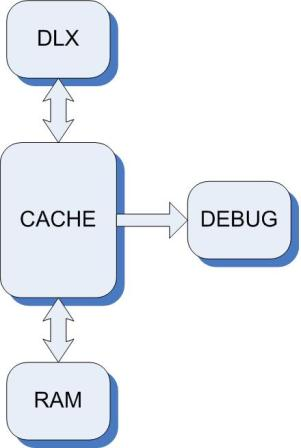
\includegraphics{img/01-interfacce_schema_generale.jpg}
 \caption{Interfacce della memoria cache}
 \label{fig:int_gen}
\end{figure}


L'interfaccia verso il micropocessore, mostrata in Fig. \ref{fig:int_dlx}, consente a quest'ultimo di accedere ai dati memorizzati all'interno della cache. 

\begin{figure}[!h]
 \centering
\includegraphics{img/dlx-cache.jpg}
 \caption{Interfaccia della memoria cache verso il processore DLX}
 \label{fig:int_dlx}
\end{figure}

In particolare sono presenti i seguenti segnali:
\begin{itemize} %i nomi dei comandi non sono esatti: vanno sostituiti
\item \textbf{Address[31-2]}: indirizzi a 32 bit emessi dal microprocessore
\item \textbf{Data[32-0]}: bus dati con parallelismo 32bit 
\item \textbf{Write}: segnale per il comando di scrittura in cache
\item \textbf{Read}: segnale per il comando di lettura da cache
\item \textbf{Ready}: segnale che indica il termine dell'operazione di lettura/scrittura corrente
\end{itemize}

L'interfaccia verso la RAM, mostrata in Fig. %\ref{fig:int_ram}
, consente alla cache di recuperare i blocchi dal livello sottostante.

%\begin{figure}[!h]
% \centering
%\includegraphics{img/ram-cache.jpg}
% \caption{Interfaccia della memoria cache verso la RAM}
% \label{fig:int_dlx}
%\end{figure}

In particolare sono presenti i seguenti segnali:
\begin{itemize} %i nomi dei comandi non sono esatti: vanno sostituiti
\item \textbf{Address[31-2]}: indirizzi a 32 bit emessi dalla cache
\item \textbf{Data[32-0]}: bus dati con parallelismo 32bit 
\item \textbf{Write}: segnale per il comando di scrittura in RAM
\item \textbf{Read}: segnale per il comando di lettura dalla RAM
\item \textbf{Ready}: segnale che indica il termine dell'operazione di lettura/scrittura corrente
\end{itemize}

Si noti che la cache non \`e a conoscenza del componente posto al livello superiore. Vista la simmetria delle due interfacce \`e quindi possibile sostituire la RAM con un ulteriore livello di cache. inserendo quindi pi\`u livelli di cache all'interno del processore.\\
\`E presente infine una terza interfaccia verso l'esterno, utilizzata per monitorare lo stato interno della cache e poter quindi eseguire il debug.
I segnali disponibili verranno definiti nel seguito.\\
Si ipotizza che la memoria cache progettata non sia impiegata in sistemi multimaster. Per tale motivo non si considereranno problematiche inerenti alla presenza di un controllore di memoria e all'invalidazione delle linee.










